\documentclass[aps,prl,reprint,superscriptaddress,floatfix]{revtex4-1}

%--- PACKAGES ---%
% \usepackage[T1]{fontenc}
\usepackage{graphicx}
\usepackage[usenames,dvipsnames]{color}
\usepackage{amsmath,amssymb}
\usepackage{bm}
\usepackage{upgreek}
\usepackage{xspace}
\usepackage{units}
\usepackage{hhline}
\usepackage[vskip=0pt]{quoting}
\usepackage[colorlinks,urlcolor=blue,citecolor=blue,linkcolor=blue]{hyperref}
\graphicspath{{figures/}}
\renewcommand{\arraystretch}{1.5}

%--- TEXT SHORTCUTS ---%
\newcommand{\etal}{et~al.\xspace}
\newcommand{\Rb}{$^{87}$Rb\xspace}
\newcommand{\qmagic}{q_{\text{magic}}\xspace}
\newcommand{\qRmagic}{q_{R,\text{magic}}\xspace}
% \newcommand{\lundblad}{Phys. Rev. Lett. \textbf{118}, 2xxxxx (2017)}
\newcommand{\lundblad}{arXiv:1706.xxxx}

%--- TEXT OPERATORS ---%
\newcommand{\reffig}[1]{\mbox{Fig.~\ref{#1}}}
\newcommand{\refeq}[1]{\mbox{Eq.~(\ref{#1})}}
\newcommand{\refsec}[1]{\mbox{Sec.~(\ref{#1})}}
\newcommand{\note}[1]{\textcolor{ForestGreen}{[\textrm{#1}]}} % Make editorial notes red

%--- MATH OPERATORS ---%
\newcommand{\upd}{\text{d}}
\newcommand{\totalD}[2]{\frac{\upd #1}{\upd #2}}
\newcommand{\partialD}[2]{\frac{\partial #1}{\partial #2}}
\newcommand{\vecop}[1]{\hat{\mathbf{#1}}\xspace}
\newcommand{\expect}[1]{\langle #1 \rangle}
\newcommand{\abs}[1]{\vert #1 \vert \xspace}
\newcommand{\bra}[1]{\langle #1 \vert \xspace}
\newcommand{\ket}[1]{\vert #1 \rangle \xspace}
\newcommand{\braket}[2]{\langle #1 \vert #2 \rangle \xspace}
\newcommand{\vect}[1]{\mathbf{#1}\xspace}
\newcommand{\uvect}[1]{\hat{\mathbf{#1}}\xspace}
\newcommand{\epvec}{\hat{\mathbf{\epsilon}}\xspace}
\newcommand{\jvect}{\mathbf{\tilde{E}}\xspace}
\newcommand{\ham}{\mathcal{H}}

% Underscores in text (from http://tex.stackexchange.com/a/38720)
\catcode`_=12
\begingroup\lccode`~=`_\lowercase{\endgroup\let~\sb}

\begin{document}

\title{Continuously observing the spectrum of a dynamically decoupled spin-1 quantum gas}

\author{R.\,P.~Anderson}
\author{M.\,J.~Kewming }
\author{L.\,D.~Turner}
\affiliation{School of Physics \& Astronomy, Monash University, Victoria 3800, Australia.}

\date{\today}

\begin{abstract}
Quantum states and spectra can be made sensitive to a particular measurand whilst simultaneously impervious to parasitic fluctuations of an environment.
Here we use an atom-light interface with minimal backaction to probe the spectrum of a radiofrequency-dressed spin-1 quantum gas continuously and in-situ.
The dressing amplitude sets the radiofrequency band in which oscillating magnetic fields manifest a linear measurand, and we probe the energy spectrum while the system evolves unitarily.
By varying a symmetry-breaking parameter of the Hamiltonian, we find a regime in which two of the dressed states are maximally insensitive (up to fourth-order) in magnetic field fluctuations that are slow compared to the dressed-state splittings.
Moreover, we demonstrate the predictive power of our continuous probe to optimize the dynamical decoupling and tune the measurement band \note{The optimum dynamically decoupled case would coincide with the longest decoherence time, this seems to be the trend in the literature}.
This robust system shares the useful hallmarks of quantum metrology platforms; the states are thus termed ``synthetic clock'' states in a complementary result by Lundblad~\etal (\lundblad) and are candidates for band-tunable magnetometry and emulation of quantum magnetism in solid-state systems. 
\end{abstract}

\maketitle

% \section{Introduction}
% \label{sec:introduction}
From Hahn echoes to contemporary dynamical decoupling, abrupt, discrete rotations have been used to protect spin superpositions from inhomogeneities and parasitic fluctuations, prolonging quantum coherence and circumventing deleterious energy shifts \cite{biercuk_optimized_2009,lange_universal_2010,bluhm_dephasing_2011}.
A complementary strategy is to replace the pulse train with an uninterrupted coupling of `bare' spin states, thus admitting new `dressed' spin eigenstates, with a modified quantization direction, spectrum, and coupling, which too are protected from unwanted artifacts of their environment~\cite{fanchini_continuously_2007}.
This \textit{continuous} dynamical decoupling (CoDD) has proven useful across multiple platforms including nitrogen-vacancy centers~\cite{hirose_continuous_2012,loretz_radio-frequency_2013,cai_robust_2012,*cai_long-lived_2012,golter_protecting_2014} and superconducting qubits, and forms the basis for creating protected qubit~\cite{aharon_general_2013} and decoherence-free~\cite{facchi_quantum_2002,*facchi_unification_2004} subspaces.
Weak continuous measurement is a powerful instrument for appraising and refining dynamical decoupling in real time; to probe stochastic evolution, improve metrological bandwidth, or realize quantum feedback schemes~\cite{vijay_stabilizing_2012}.
Here we use minimally perturbative \note{dispersive} optical readout of a `bare' spin component $\hat{F}_x$ to measure the real-time spectrum of a continuously decoupled spin-1 using Fourier spectroscopy. 
Recently, Fourier spectroscopy was used to measure band structures of a spin-orbit coupled BEC \cite{valdes-curiel_fourier_2017} comprised of numerous single-shot experiments.
The rich continuous time-frequency domain data in our experiment reveal not only multiple dressed-state splittings and their relative immunity to noise, but also dressed state coherences and coupling strengths.
This potent ability to estimate the eigenspectrum of a multi-level dressed system reveals features absent in spin-1/2 or composite spin-1/2 qubit systems; principally, we identify a regime in which a subspace of the dressed system is maximally decoupled from noise amplitude fluctuations $\propto \hat{F}_z$.
This subspace is spanned by two of the dressed states, termed `synthetic clock states' in a co-submission by Lundblad~\etal (\lundblad).
The low-frequency magnetic stability and high-bandwidth detection of these states is immediately applicable to band-tunable (ac) magnetometry~\cite{hirose_continuous_2012,loretz_radio-frequency_2013,ockeloen_quantum_2013,*horsley_frequency-tunable_2016} and experiments preparing delicate spin-entangled many-body states~\cite{stamper-kurn_spinor_2013}; whereas the unconventional cyclic coupling of all $2F+1$ dressed states could be applied to emulation of frustrated quantum spin chains~\cite{mikeska_one-dimensional_2004}.
% The spin-1 asymmetry arising from $\hat{F}_z^2$...
% The eigenstates produced by CoDD are simply the familiar 'dressed states' of atomic physics.

% Weak continuous measurements based on dispersive probes have found broad application in NV centers, superconducting qubits \note{single spin readout (not ensemble), requiring repeated preparation and measurement to obtain a spectrum}, and cold atoms \note{with bare states, magnetometry, spin dynamics, tomography and spin squeezing}... but have not been used in concert with CoDD to date.

Atomic Zeeman states $\ket{m_z=-1,0,1}$ in a magnetic field $B_z \vect{e}_z$ can be decoupled from amplitude fluctuations in $B_z$ by applying a radiofrequency (rf) field perpendicular to the quantization direction $z$, of amplitude $B_{\text{rf}} \vect{e}_x$, and oscillating near the splitting of the `bare' Zeeman states $\omega_L \equiv (E_{m_z=+1}-E_{m_z=-1})/2\hbar$, the Larmor frequency.
At low magnetic fields, the degeneracy of the composite spin-$1/2$ systems~\cite{majorana_atomi_1932} \note{why are we citing Majorana?} renders the spin-1 behavior identical to CoDD in spin-$1/2$ qubits.
The spin is quantized along $x$ in a frame rotating with the radiofrequency $\omega_{\text{rf}}$, i.e. the eigenstates of $\ham_{\text{rwa}} = \Delta \hat{F}_z + \Omega \hat{F}_x$ are $\ket{m_x=-1,0,1}$, with energies $m_x \hbar \sqrt{\Omega^2 + \Delta^2}$, where $\Delta = \omega_{\text{rf}}-\omega_L$ is the detuning and $\Omega = \gamma B_{\text{rf}} / 2$ is the Rabi frequency.
The rf dressing reduces the leading-order linear sensitivity of the `bare' state energies ($\omega_L \approx \gamma B_z$ where $\gamma$ is the gyromagnetic ratio) to magnetic field variations $\delta B_z$ to quadratic sensitivity, via the detuning $\Delta$.
The spin character and symmetries are otherwise unchanged; magnetic fields along $y$ or $z$ oscillating near the Rabi frequency drive transitions $\ket{m_x=-1} \leftrightarrow \ket{m_x=0}$ and $\ket{m_x=0} \leftrightarrow \ket{m_x=+1}$, the basis for ac magnetometry~\cite{hirose_continuous_2012} or concatenated CoDD to mitigate fluctuations in $\Omega$ on the spectrum and coherences~\cite{cai_robust_2012}.

However, any $\hat{F}_z^2$ interaction -- arising from nonlinear Zeeman~\cite{ramsey_molecular_1956}, microwave ac-Stark~\cite{gerbier_resonant_2006}, or tensor light~\cite{smith_continuous_2004} shifts -- raises the degeneracy of the $\ket{m_z=-1} \leftrightarrow \ket{m_z=0}$ and $\ket{m_z=0} \leftrightarrow \ket{m_z=+1}$ transitions, and breaks the symmetry of $\ham_{\text{rwa}} = \Delta \hat{F}_z + \Omega \hat{F}_x + q \hat{F}_z^2$, where $q \equiv (E_{m_z=+1} + E_{m_z=-1} - 2 E_{m_z=0})_{\Omega=0}/2\hbar$.
\begin{figure}
    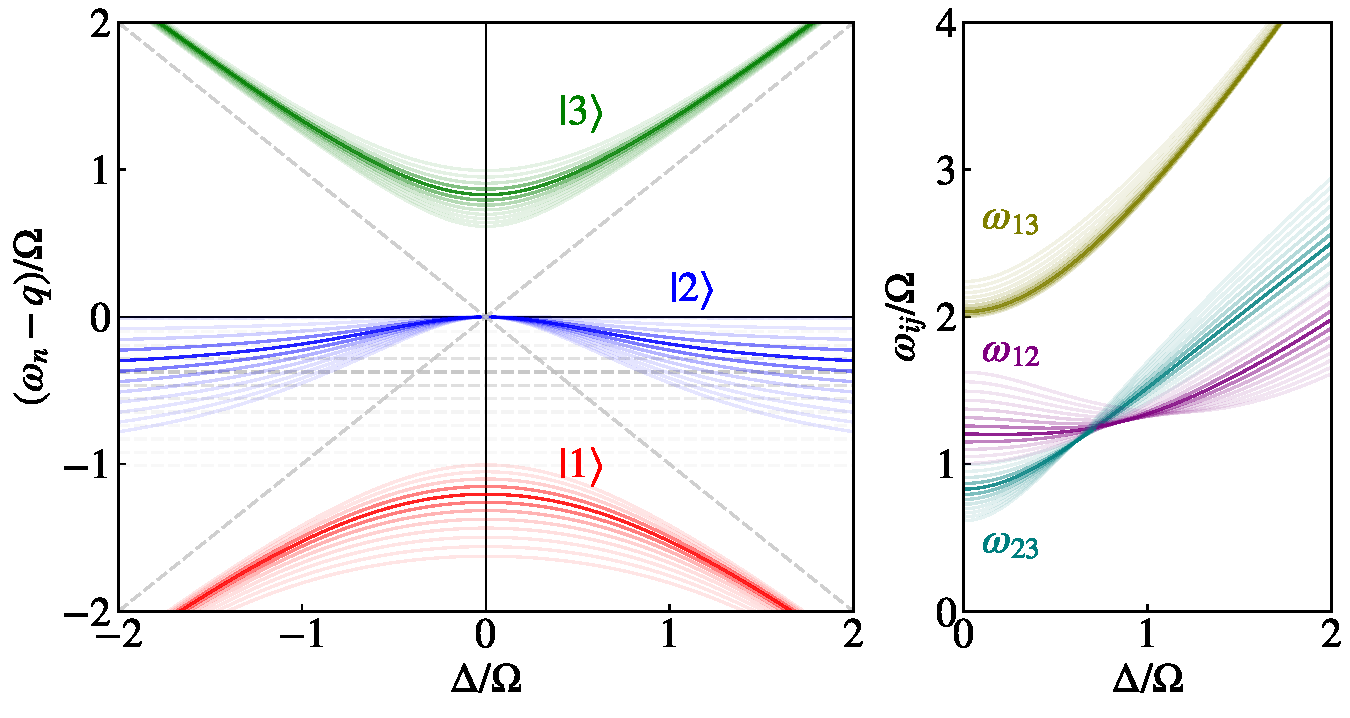
\includegraphics[width=\columnwidth]{figure_1.pdf}
    \caption{
    \label{fig:eigensystem_schematic}
        % (Color online)
        Energy spectrum and splittings of a radiofrequency coupled spin-1 for various $q \in [0,\Omega]$.
        The transparency of each curve is proportional to the distance of $q/\Omega$ from $\qRmagic$ in \refeq{eq:qRmagic}.
        (Left) Energies $\omega_n$ of dressed states $\ket{n}=\ket{1}$, (red) $\ket{2}$ (blue), and $\ket{3}$ (green) normalized to the rf-coupling strength (Rabi frequency) $\Omega$ as a function of detuning $\Delta=\omega_{\text{rf}}-\omega_L$,
        Dashed lines indicate the energies of uncoupled states ($\Omega=0$) in a frame rotating at $\omega_{\text{rf}}$.
        (Right) Splittings $\omega_{ij}$ of dressed states $\ket{i}$ and $\ket{j}$ as a function of detuning.
        When $q/\Omega=\qRmagic$ (bold curves), energies $\omega_1$ and $\omega_2$ share the same curvature, and their difference $\omega_{12}$ (right, purple) is minimally sensitive to detuning and thus magnetic field variations.
    }
\end{figure}
This yields dressed eigenstates $\{\ket{1}, \ket{2}, \ket{3}\}$ that are no longer $\text{SO}(3)$ rotations of the bare Zeeman states $\ket{m_z}$, but have nematic order, and an eigenspectrum $\omega_i(\Delta) = E_{\ket{i}}/\hbar$ shown in \reffig{fig:eigensystem_schematic} (left) for $q \in [0, \Omega]$.
Moreover, the coupling of these dressed states is markedly different: the spin operators $\hat{F}_{x,y,z}$ in the dressed basis span more of $\text{SU}(3)$ for $q \neq 0$, e.g. $\bra{i} \hat{F}_x \ket{j}$ has a non-zero projection onto the fourth Gell-Mann matrix $Q_{x^2-y^2}$ \note{why is this the fourth Gell-mann matrix? $\lambda_{4}$ would be more common} signifying the direct coupling of dressed states $\ket{1}$ and $\ket{3}$.
The dressed-state transitions are thus cyclic and non-degenerate (\reffig{fig:eigensystem_schematic}(right)), characterized by a dressed Larmor frequency
\begin{align}
\label{eq:dressed_larmor}
    \omega_D \equiv (\omega_3 - \omega_2)_{\Delta=0}/2 &= (\omega_{12} + \omega_{23})_{\Delta=0}/2 \notag\\ &= \sqrt{\Omega^2 + q_D^2}\, ,
\end{align}
and dressed quadratic shift
\begin{align}
\label{eq:dressed_quadratic}
    q_D &\equiv (\omega_3 + \omega_1 -2\omega_2)_{\Delta=0}/2 \notag\\
        &= (\omega_{23}-\omega_{12})_{\Delta=0}/2 \notag s\\ 
        &= -q/2 \, .
 \end{align}
The curvature of the dressed state energies $\omega_i(\Delta)$ depends on the normalized quadratic shift $q_R = q/\Omega$, and is equal for states $\ket{1}$ and $\ket{2}$ when 
% $q_R=\qRmagic = \sqrt{(3\sqrt{2} - 4)/2} \approx 0.348$,
\begin{align}
\label{eq:qRmagic}
    q_R = \qRmagic = \sqrt{(3\sqrt{2} - 4)/2} \approx 0.348 \, ,
\end{align}
resulting in vanishing quadratic dependence of their transition frequency $\omega_{12}=\omega_2 - \omega_1$ on $\Delta$~\footnote{
    The curvature of the dressed-state energies is evaluated using perturbation theory. In particular, the dimensionless curvature of $\omega_{12}$ is $\partial^2(\omega_{12}/\Omega)/\partial(\Delta/\Omega)^2 = \Omega \, \partial^2\omega_{12}/\partial \Delta^2 = -(3 q_R \sqrt{4 + q_R^2} - q_R^2 - 2)/(2 \sqrt{4 + q_R^2})$.
    For $q_R = 0$, we recover the spin-1/2 result, $\Omega\, \partial^2\omega_{12}/\partial \Delta^2 = 1$}.
The leading-order sensitivity of these states to field variations $\delta B_z$ at $\qRmagic$ is quartic~\footnote{
    We take $\Delta = -\gamma \, \delta B_z$ for $|\Delta | \leq 2\Omega$ ($| \delta B_z | \leq B_{\text{rf}}/2$) and $| \partial q / \partial \Delta | \approx | \gamma^{-1} \partial q / \partial B_z | = |2 B_z q_Z / \gamma| \ll 1$, valid to $10^{-3}$ for the field strengths $B_z \lesssim \unit[5]{G}$ used here, resulting in vanishing third-order derivatives of $\omega_i$ with respect to detuning. 
    In general, the variation of $q$ with $\Delta$ (or $\delta B_z$) can be accounted for using the Breit-Rabi equation, leading to a residual linear and cubic variation of $\omega_{12}$ with $\delta B_z$, and a small correction to $\qRmagic$ in \refeq{eq:qRmagic}.},
amounting to their optimal CoDD and we join in Lundblad \etal in terming them synthetic clock states in this configuration.

% It is this dressed spectrum and the optimal CoDD we probe using continuous weak measurement in the remainder of this paper.
We experimentally demonstrate this optimal CoDD using continuous measurement of a spin-1 non-degenerate quantum gas.
Our spinor quantum gas apparatus~\cite{wood_magnetic_2015} and Faraday atom-light interface are described in greater detail elsewhere~\cite{jasperse_magic-wavelength_2017}.
We prepare an ultracold gas ($\sim \unit[1]{\upmu K}$) of approximately $10^6$ \Rb atoms in a crossed-beam optical dipole trap ($\lambda=\unit[1064]{nm}$).
The three Zeeman states $\ket{m_z=-1,0,+1}$ of the lowest hyperfine ($F=1$) ground state are coupled using a radiofrequency field with $\Omega/(2\pi) \leq \unit[100]{kHz}$, generated by a single-turn coil placed immediately atop the glass vacuum cell, fed by an amplified radiofrequency source generated using direct-digital synthesis.
A component of the collective spin transverse to the static magnetic field direction (along $z$) rotates the polarization of an off-resonant probe beam via the paramagnetic Faraday effect; shot-noise limited polarimetry of the optical probe in a bandwidth near the Larmor frequency $\omega_L$ thus measures $\expect{\hat{F}_x}$.

Weak continuous measurement using the paramagnetic Faraday effect has been used to observe spin-mixing dynamics of a polar spinor condensate~\cite{liu_quantum_2009} and perform quantum state tomography~\cite{smith_continuous_2004,*smith_efficient_2006}.
Similar polarimetry-based dispersive probes have been used to measured hyperfine Rabi oscillations of the collective clock-transition pseudospin~\cite{chaudhury_continuous_2006}; modulating the birefringence of the atomic ensemble near baseband, resulting in polarization rotation oscillating at the Rabi frequency.

To probe the dressed state spectrum and coherences, we prepare a superposition of dressed states by suddenly turning on the Rabi coupling $\Omega$ at $t=0$, projecting the polarized collective spin $\ket{m_z=-1}$ onto $\ket{\psi(t=0)} = \sum_i c_i \ket{i}$.
The total magnetic field in the laboratory frame used to affect this control is $\vect{B}(t \geq 0) = -B_{\text{rf}} \cos (\omega_{\text{rf}} t) \vect{e}_x + B_z(t) \vect{e}_z$, where $B_z(t)$ varies slowly compared to $\Omega$.
The resulting Faraday signal is presented in the time-frequency domain using the short-time Fourier transform (spectrogram), revealing the rich frequency and amplitude modulation related to the dressed state energies, coherences, and coupling strengths.
For example, with no deliberate variation of the Rabi frequency or detuning, we observe the spectrogram amplitude shown in \reffig{fig:static_coupling}.
Strong amplitude modulation of the Faraday signal is apparent from the three upper and lower sidebands, each pair equidistant from the carrier frequency at $f_{\text{rf}} = \omega_{\text{rf}}/(2\pi)$. 
\begin{figure}
    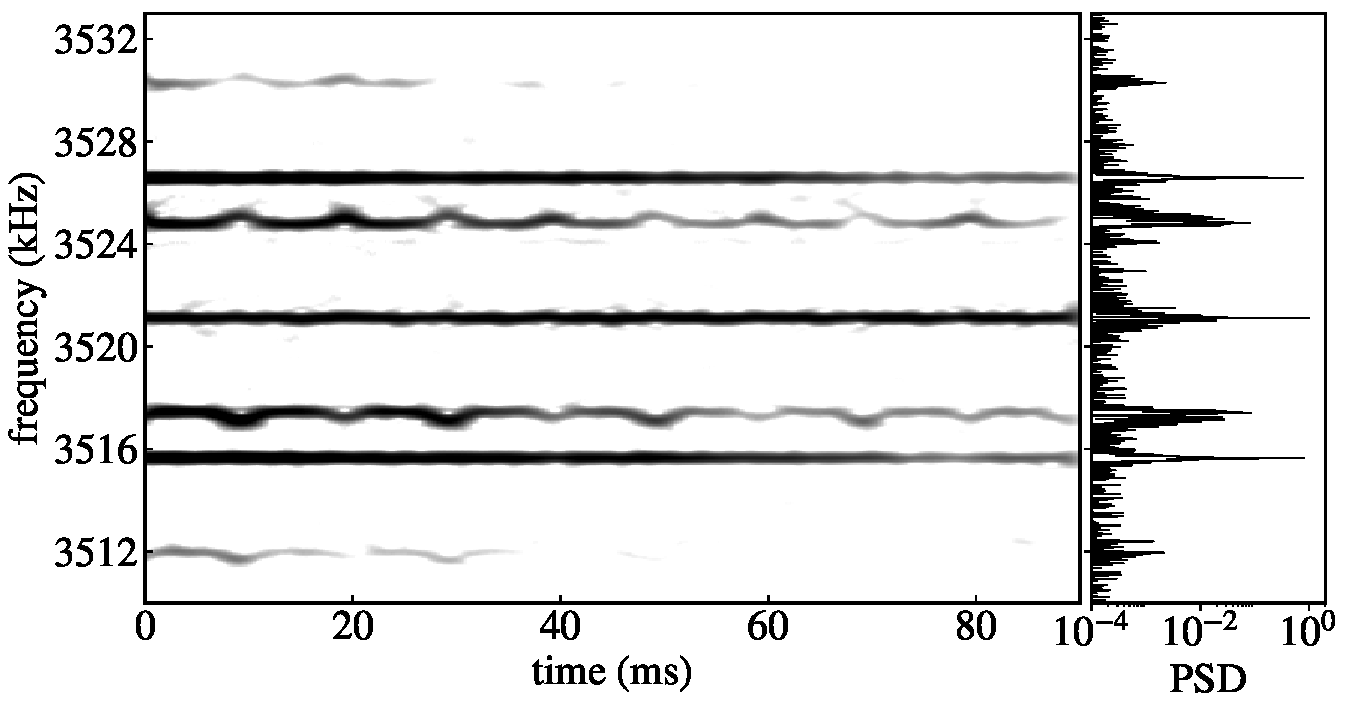
\includegraphics[width=\columnwidth]{figure_2.pdf}
    \caption{
    \label{fig:static_coupling}
    Continuous measurement of the dressed energy spectrum for $q_R = 0.402(3)$, $f_{\text{rf}}=\unit[3.521]{MHz}$ and $B_0=\unit[5.013]{G}$ (left) and a periodogram of the $\unit[100]{ms}$ long signal (right). 
    (Inset) The dressed state energy diagram for resonant coupling ($\abs{\Delta} \ll \Omega$); the mean and difference of transition frequencies $\omega_{12}$ and $\omega_{23}$ is the dressed Larmor frequency $\omega_D$ and quadratic shift $q_D$, respectively.
    The upper sidebands about the carrier at $f_{\text{rf}}$ are associated with the $\omega_{13}$ (gold), $\omega_{23}$ (turquoise), and $\omega_{12}$ (lavender) transitions.  
    % The upper sidebands about the carrier at $f_{\text{rf}}$ associated with each of the three transitions are indicated by gold ($\omega_{13}$), turquoise ($\omega_{23}$), and lavender ($\omega_{12}$) annotations.  
    Magnetic field fluctuations $\delta B_z = \delta B_{\text{ac}}(t)$ of amplitude $\unit[1.4]{mG}$ induced by mains power are manifest as asymmetric frequency modulation of the $\omega_{13}$ and $\omega_{23}$ sidebands, while the $\omega_{12}$ transition remains relatively unaffected.
    The corresponding spectral peaks have linewidths $\unit[102]{Hz}$, $\unit[97]{Hz}$, and $\unit[24]{Hz}$, respectively.
    The $\omega_{12}$ linewidth is transform-limited, whereas the broadened peaks of the less decoupled $\omega_{23}$ transition exhibit a skew (third-moment) of $\unit[84]{Hz}$ (upper sideband) and $-\unit[100]{Hz}$ (lower sideband).
    }
\end{figure}
Each pair of sidebands corresponds to a dressed state transition $\ket{i} \leftrightarrow \ket{j}$; centered at $f_{\text{rf}} \pm f_{ij}$ where $f_{ij} = \omega_{ij}/(2\pi)$, the frequency of the transition.
In this way, the spectrogram is a calibration-free, real-time measurement of the dressed state spectrum.
Restricting attention to the upper sidebands, the two closest to the carrier are ladder-type transitions $\omega_{12}$ and $\omega_{23}$ have similar amplitudes and lifetimes, with frequency separations $\omega_D \pm q_D$ from the carrier, respectively, for near-resonant coupling of the bare Zeeman states ($\abs{\Delta} \ll \Omega$).
The third, weaker sideband near $2\omega_D$ above the carrier is a signature of the cyclic $\ket{1} \leftrightarrow \ket{3}$ transition, permitted only when $q\neq 0$.
% $\omega_D/(2\pi) = \unit[4611(2)]{Hz}$, $q_D/(2\pi) = \unit[910(5)]{Hz}$, $\Omega/(2\pi) = \unit[4520(2)]{Hz}$, $\omega_{\text{rf}}/(2\pi) = f_{\text{rf}} = \unit[3.521]{MHz}$, 
No attempt was made to shield the apparatus from parasitic magnetic fields, and mains power induced magnetic field noise causes a temporally varying $\delta B_z = \delta B_{\text{ac}}(t)$ at the line frequency of $\unit[50]{Hz}$ and its odd harmonics, of peak-to-peak amplitude $\sim\unit[1.4]{mG}$ ($\unit[1]{kHz}$ in frequency units of detuning).
For these data $q_R = 0.402(3)$ each dressed transition is affected by the magnetic fluctuations differently; the sidebands corresponding to the $\omega_{13}$ and $\omega_{23}$ transitions exhibit asymmetric frequency modulation, whereas the $\omega_{12}$ transition remains relatively unaffected.
This is signified by skewed peaks in the periodogram (\reffig{fig:static_coupling}, right), e.g. the $\omega_{23}$ sidebands have a third-moment of $\unit[84]{Hz}$ (upper) and $-\unit[100]{Hz}$ (lower), and a linewidth that is $4$ times broader than the transform-limited peak of the $\omega_{12}$ transition ($\unit[24]{Hz}$ second-moment).
\begin{figure}
    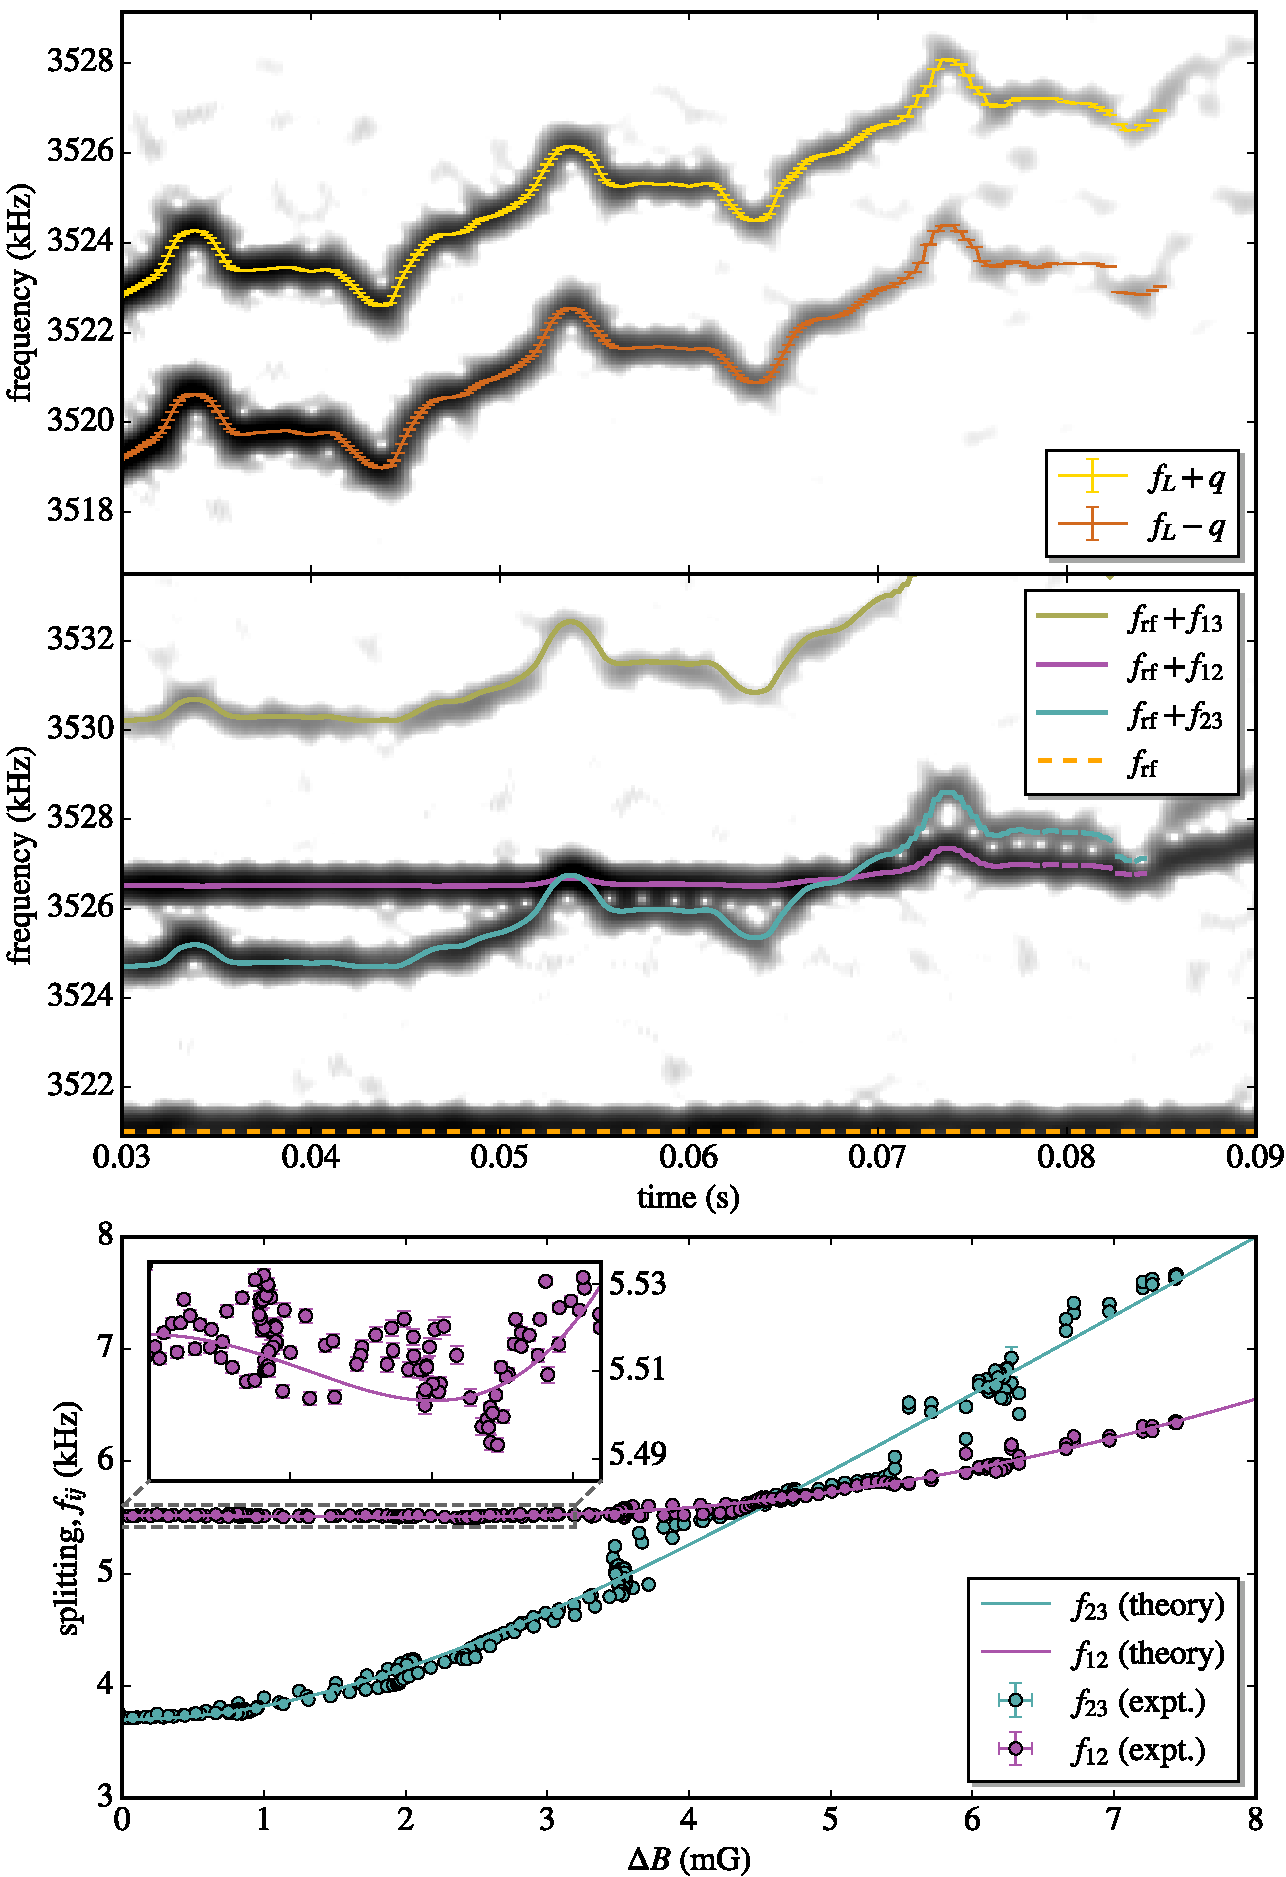
\includegraphics[width=\columnwidth]{figure_3.pdf}
    \caption{
    \label{fig:acquisition_pipeline}
        % (Color online)
        Real-time CoDD observation for $q_R = 0.402(3)$.
        % ($f_{\text{rf}}=\unit[3.521]{MHz}$, $B_0=\unit[5.013]{G}$).
        (a) and (b) are spectrograms of a continuous weak measurement of $\expect{\hat{F}_x}$.
        (a) Magnetometry of the bare Zeeman states ($\Omega=0$) used to calibrate $B_z(t) = B_0 + \delta B_z(t)$ over the interrogation interval, in which the field [detuning] varies over a range $\sim B_{\text{rf}}$ [$2\Omega$].
        % and the spinor gas is left to Larmor precess in the absence of a dressing field ($\Omega = 0$).
        We numerically track the bare Zeeman splittings (gold/orange) to determine the instantaneous Larmor frequency $f_L(t)$ and quadratic shift $q(t)$.
       (b) The field is swept over the same range but the rf dressing is applied ($\Omega > 0$).
       Three sidebands above (shown) and below the carrier at $f_{\text{rf}}=\unit[3.521]{MHz}$ (dashed, orange) reveal the dressed state splittings $f_{ij} = \omega_{ij}/(2\pi)$.
       (c) A parametric plot of $f_{12}(t)$ and $f_{23}(t)$ versus $\delta B_z(t)$ by combining analysis of (a) and (b).
       Solid curves in (b) and (c) are theoretical splittings from an eigenspectrum calculation, provided only $f_{\text{rf}}$, $B_z(t)$, and $\Omega$, i.e. no free parameters.
       Variation of the synthetic clock transition $f_{12}$ for $0 \leq \delta B_z \leq B_{\text{rf}}/4 = \unit[3.2]{mG}$ (c, inset).
    }
\end{figure}
The amplitude of each sideband is proportional to the corresponding dressed-state coherence $c_i^* c_j = \rho_{ij}$, and the dressed state coupling strength induced by the relevant spin projection operator $\hat{F}_{x,y,z}$.
\begin{table*}[t]
    \caption{Upper sidebands of the carrier (at $\omega_{\text{rf}}$) of the Faraday rotation signal $\propto \expect{\hat{F}_x}$ of an arbitrary dressed state superposition driven on resonance ($\Delta = 0$).
    Frequency and phase are reported relative to the carrier, along with the transition that each sideband corresponds to.
    For the initial state $\ket{\psi(t=0)}=\ket{m_z=-1}$, the sideband frequencies and amplitudes can be concisely expressed in terms of the dressed Larmor frequency $\omega_D$ and quadratic shift $q_D$. 
    For each upper sideband, there is a lower sideband of the same amplitude, relative frequency and opposite relative phase.
    \label{tab:sidebands}
    }
    \begin{ruledtabular}
    \begin{tabular}{ccccc}
    transition & frequency & $\omega_{ij} - \omega_{\text{rf}}$ ($\Delta=0$) & amplitude ($\Delta = 0$) & amplitude ($\Delta = 0$, $\ket{m_z=-1}$) \\ \hline
     (carrier) & $\omega_{\text{rf}}$ & 0 & $(\bra{3} \hat{F}_x \ket{3} - \bra{1} \hat{F}_x \ket{1}) (\rho_{33} - \rho_{11})$  & $q_D \Omega/(2 \omega_D^2)$ \\
     $\ket{1} \leftrightarrow \ket{2}$ & $\omega_{\text{rf}} + \omega_{12}$ & $\omega_D+q_D$ & $-2i \bra{1} \hat{F}_y \ket{2} \text{Re}\{\rho_{12}\} = -2 \bra{2} \hat{F}_z \ket{3} \text{Re}\{\rho_{12}\}$ & $\Omega/(4 \omega_D)$ \\
     $\ket{2} \leftrightarrow \ket{3}$ & $\omega_{\text{rf}} + \omega_{23}$ & $\omega_D-q_D$ & $2i \bra{2} \hat{F}_y \ket{3} \text{Re}\{\rho_{23}\} = 2 \bra{1} \hat{F}_z \ket{2} \text{Re}\{\rho_{23}\}$ & $\Omega/(4 \omega_D)$ \\
     $\ket{1} \leftrightarrow \ket{3}$ & $\omega_{\text{rf}} + \omega_{13}$ & $2\omega_D$ & $2 \bra{1} \hat{F}_x \ket{3} \text{Re}\{\rho_{13}\}$ & $q_D \Omega/(4 \omega_D^2)$
    \end{tabular}
    \end{ruledtabular}
\end{table*}
For near-resonant coupling of the bare Zeeman states, an analytic expression for the amplitudes can be obtained, summarized in Table~\ref{tab:sidebands}.
These depend on the initial projection onto the dressed basis, which if known permits continuous measurement of all coupling strengths in the dressed basis, an analogue of Hamiltonian parameter estimation \note{process tomography/ Hamiltonian learning}.
Alternatively, independent characterization of the dressed state couplings~\cite{lundblad_synthetic_2017} permits real-time measurement of the dressed density matrix, an analogue of quantum state estimation.

To appraise the relative CoDD of dressed state transitions, and their dependence on the quadratic shift $q_R$, 
we varied the magnetic field over a wider range than in \reffig{fig:static_coupling}, sweeping the bias magnetic field along $z$ over a range $B_{\text{rf}}$ during the measurement interval.
\note{We should tread lightly here on this previous comment. We should avoid drawing attention to the question ``If it is optimally decoupled, then it should show the longest decoherence time. Have you done this?''}
The control field $B_z(t) = B_0 + \alpha t + B_{\text{ac}}(t)$, where $\alpha = \unit[128]{mG/s}$ is the linear sweep rate; the resulting detuning variation is of order $2\Omega$ (\textit{cf.} the domain of~\reffig{fig:eigensystem_schematic}).
% To appraise the robustness of the rf-dressed states to varying magnetic fields,
% we apply a time dependent $\delta B_z(t)$ and observe the dynamical change in the frequency composition of the Faraday signal using the short-time Fourier transform, or spectrogram.
For each realization (or `shot') of the experiment, we directly calibrate $B_z(t)$ using magnetometry of the bare Zeeman states; an rf $\pi/2$-pulse (rather than continuous coupling) initiates Larmor precession of the collective spin in the $x$--$y$ plane, and the Faraday signal is composed of two tones at $\omega_\pm = \omega_L \pm q$, the bare Zeeman splittings (\reffig{fig:acquisition_pipeline}, top).
For $q \, \tau_f \geq 2\pi$, where $\tau_f$ is the length of the overlapping spectrogram windows, the two tones are spectrally resolved and their mean and difference yields the instantaneous $\omega_L(t)$ and $q(t)$, the former of which is used to find $\delta B_z(t)$ (and $\Delta(t)$) by inverting the Breit-Rabi equation~\cite{ramsey_molecular_1956}~\footnote{
    The experiment is synchronized to the mains power line; the harmonic composition of which varies little between contiguous shots ($\unit[20]{s}$ apart), and thus the measured $\delta B_z(t)$ and $q(t)$ from the calibration \note{fiducial?} shot serve as a good proxy for the values experienced by the atoms in the subsequent CoDD shot.
}.

We measured the dressed spectrum for a range of resonant magnetic fields $B_0 \in [3.549, 5.568]\unit{G}$ (applied rf frequency $f_{\text{rf}} \in [2.493, 3.911]\unit{MHz}$), with a fixed Rabi frequency of $\Omega/(2\pi) = \unit[4.505(3)]{kHz}$ ($B_{\text{rf}} = \unit[12.83(1)]{mG}$).
For each resonant field $B_0$, we ensured the Rabi frequency was fixed by measuring the voltage drop across the coil at $f_{\text{rf}}$ with a lock-in amplifier which -- in concert with an impedance analyzer -- could be used to ensure the rf current in the coil and thus $B_{\text{rf}}$ and $\Omega$ were constant.
The Rabi frequency was ultimately measured using the atoms, by analyzing a subset of the dressed energy spectrum during the magnetic field sweep when $\abs{\Delta}/(2\pi) \leq \unit[100]{Hz}$.
The measured Rabi frequencies had a standard deviation $\sigma(\Omega) = \unit[9.4]{Hz}$, validating the above method.

The dressed spectrum for the swept control field with resonant field $B_0=\unit[5.013]{G}$ and $q_R=0.403(2)$ is shown in~\reffig{fig:acquisition_pipeline}b.
The instantaneous dressed state splittings for all three transitions were predicted with no free parameters, and are plotted atop the spectrogram data, showing excellent agreement with the measured sidebands.
Because $\delta B_z(t)$ is non-linear and non-monotonic in time, we use the raw time series from the calibration ($\Omega=0$) and CoDD shots to form parametric $(\delta B_z(t), f_{ij}(t))$ data, by tracking the instantaneous peaks in each spectrogram.
The sensitivity of the $\ket{1} \leftrightarrow \ket{2}$ and $\ket{2} \leftrightarrow \ket{3}$ transitions to magnetic field variations are shown in \reffig{fig:acquisition_pipeline}c.
The synthetic clock transition is most insensitive; the measured [predicted] $f_{12}$ varies by $\unit[39]{Hz}$ [$\unit[26]{Hz}$] for $0 \leq \delta B_z \leq B_{\text{rf}}/4 = \unit[3.2]{mG}$ (\reffig{fig:acquisition_pipeline}c, inset).
The corresponding normalized variation in $\omega_{12}/\Omega = 8.6\times10^{-3}$ [$5.8\times10^{-3}$] across a detuning range of $0 \leq \abs{\Delta/\Omega} \leq 0.5$.
By comparison, the normalized variation at $q_R=0$ is $(\sqrt{5}-2)/2 \approx 0.118$; 14 [20] times higher than the observed [predicted] variation.
Alternatively, the normalized variation of the $\ket{m_z=\pm1} \leftrightarrow \ket{m_z = 0}$ Zeeman transitions at $q=0$ is $0.5$; 58 [86] times higher than the observed [predicted] variation in the synthetic clock transition frequency.

In the adiabatic limit, the dressed state populations remain constant and the above superposition evolves under phase acquisition $e^{-i \omega_i t}$ by each dressed state $\ket{i}$~\cite{messiah_quantum_1962}. 
We quantify the stasis of the dressed superposition using the generalized adiabatic parameter $\Gamma \equiv \abs{\vect{\Omega}(t)/\dot{\theta}(t)}$, where $\vect{\Omega} = \vect{B}_{\text{eff}} / \gamma \equiv \Omega \, \vect{e}_x + \Delta \, \vect{e}_x$ and $\tan \theta \equiv \Omega / \Delta$.
For constant coupling amplitude $\dot{\Omega} = 0$, $\dot{\theta}(t) = -\Omega \dot{\Delta}(t)/\abs{\vect{\Omega}}^2$.
For the magnetic field sweeps used here, $\Gamma > 200$ and $\sqrt{\expect{\Gamma^2}}_t \gtrsim 600$ where $\expect{\cdot}_t$ denotes the time-average over the duration of the sweep.
Nevertheless, the continuous spectra when plotted parametrically (\reffig{fig:acquisition_pipeline}c) exhibit some evidence of non-adiabatic following.
This is corroborated by numerically integrating the Schr\"{o}dinger equation of the known control Hamiltonian; the dressed state populations vary slowly (compared to $\omega_D^{-1}$) but by a few percent near minima of $\Gamma(t)$, i.e. when the sweep is least adiabatic.
\begin{figure}
    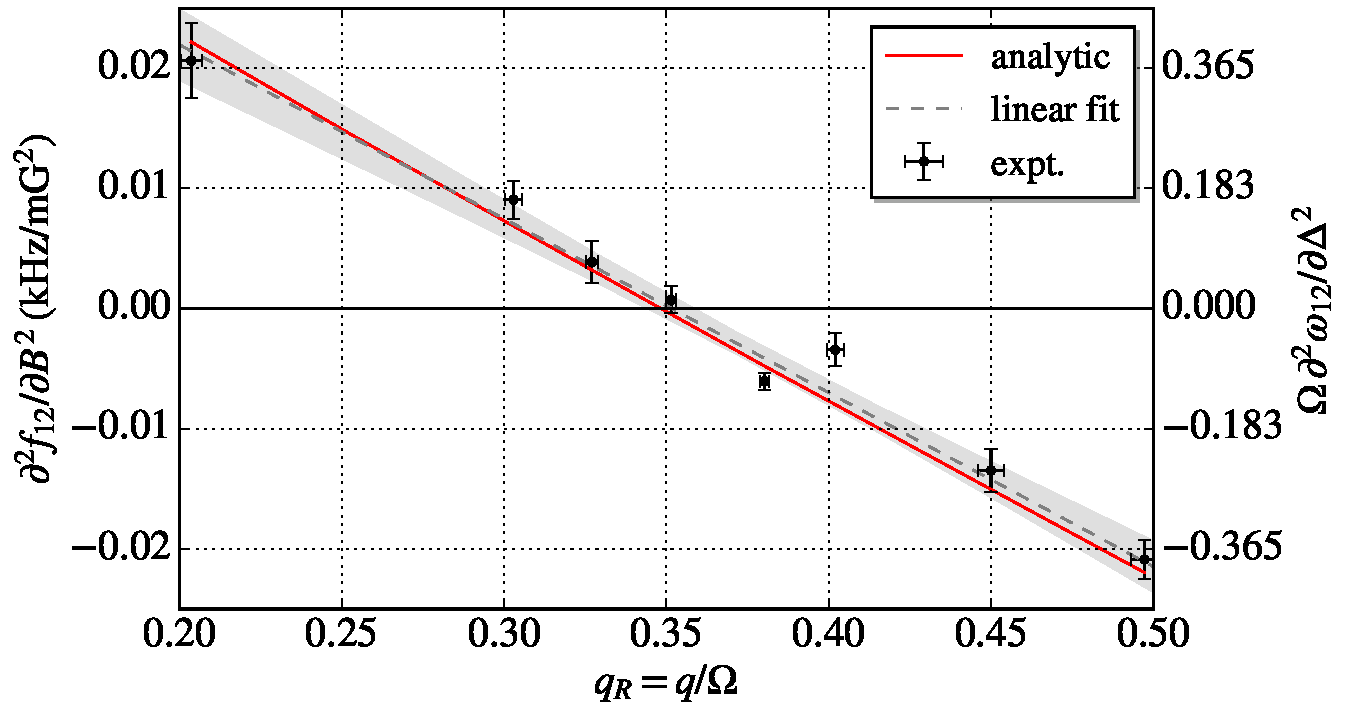
\includegraphics[width=\columnwidth]{figure_4.pdf}
    \caption{
    \label{fig:curvature_vs_qR}
        Curvature of the synthetic clock transition for normalized quadratic shifts $q_R \in [0.2, 0.5]$.
        The measured curvature (black points) was determined from polynomial fitting to $(\delta B_z, f_{12})$ data shown in \reffig{fig:acquisition_pipeline}(c).
        Vertical and horizontal error bars correspond to the standard error of the regression and uncertainty in $q_R$ (via $u(q)$ and $u(\Omega)$ at each field $B_0$), respectively.
        A linear fit (black, dashed) with 1$\sigma$ confidence band (gray, shaded) are shown, whose intercept can be used to impute $\qRmagic\text{ (expt.)} = 0.350(6)$.
        The analytic expression for the curvature (red) is consistent with the data-driven analysis of the curvature, \textit{cf.} $\qRmagic\text{ (theory)} = 0.348$.
        The left [right] vertical axis shows the curvature $\partial^2 f_{12}/\partial B_z^2$ [$\Omega\, \partial^2\omega_{12}/\partial \Delta^2$] in absolute units of $\unit{kHz/G^2}$ [dimensionless units].
        The normalized curvature is unity when $q_R=0$.
    }
\end{figure}

% The acquisition and analysis of \reffig{fig:acquisition_pipeline} was repeated for several $q_R$.  
To test the predictive power of our CoDD measurement, we inferred the curvature of the synthetic clock transition with respect to magnetic field variations, inspecting the quadratic coefficient of a polynomial fit to $(\delta B_z, f_{12})$ data.
The results of this model independent analysis are shown in~\reffig{fig:curvature_vs_qR} for $q_R \in [0.2, 0.5]$.
The curvature $\partial^2 f_{12}/\partial B_z^2$ can be predicted analytically, and varies near-linearly in $q_R$ over this range.
Accordingly, we perform linear regression to the measured curvature versus $q_R$ to infer $\qRmagic$, where the synthetic clock transition has vanishing curvature, and find $\qRmagic\text{ (expt.)} = 0.350(6)$, in agreement with the theoretical value in~\refeq{eq:qRmagic}.
The minimum curvature demonstrated here occurs at $q_R = 0.351(2)$, with a value of $\left(\partial^2 f_{12}/\partial B_z^2\right)_{\text{min}} = \unit[10^{-3}]{kHz/mG^2}$ \note{$\unit[1]{MHz/G^2}$}.
In dimensionless units -- with the splitting and detuning normalized to the Rabi frequency -- $\left(\Omega\, \partial^2\omega_{12}/\partial \Delta^2\right)_{\text{min}} = 0.02$, which is 50 times lower than the curvature of this transition for $q_R = 0$.

Despite long coherence times, the low duty cycle ($D < 0.01$) and large dead time ($T_\text{shot} \gtrsim \unit[10]{s}$) of cold quantum gas experiments make challenging achieving metrological sensitivities per unit bandwidth that are competitive with other platforms.
Here $D=0.005$ and $T_\text{shot} = \unit[20]{s}$, yet we make many more spin projection measurements (\note{$N_m$ = blah} at a shot-noise limited SNR of $10$--$100$~\cite{jasperse_magic-wavelength_2017}) than traditional cold atom experiments ($N_m = 1$ to several, e.g. absorption or dispersive imaging).
This intra-shot revelation of the time and frequency domain renders the measurement of these spectra orders of magnitude more efficient.
For example, the single spectrum shown in \reffig{fig:acquisition_pipeline} would take $\sim (10$ shots per $\delta B_z$ per $\omega_{ij} ) \times (100$ $\delta B_z$ values) $\times (3 $ transitions $\omega_{ij}) = 3000$ shots \note{$2.5$ times fewer $\delta B_z$ values than shown here}, or $\sim \unit[6\times10^4]{s} = 1000$ minutes of data acquisition.
We acquire this spectrum in a single shot \note{two shots accounting for the field calibration, but that would require $\sim 2\times$ more traditional shots}, i.e. $\unit[20]{s}$.
The data used to generate \reffig{fig:curvature_vs_qR} was acquired in only $6$ minutes.

In summary, we have demonstrated real-time measurement of continuous dynamical decoupling in a spin-1 quantum gas, and expeditious optimization of this decoupling by varying the the relative asymmetry of the Zeeman state splittings.
Continuous weak measurement via the Faraday effect yields information about the rf-dressed superposition, the dressed-state couplings and energies, simultaneously.
In this measurement regime, we do not resolve the quantum noise of the decoupled collective spin.
With a modification of the probe (atom-shot noise dominated) we could measure and affect the quantum noise dynamically,
and probing the dressed state coherences in this regime may expose non-Gaussian quantum noise geometries in a manner analogous to Ref.~\cite{colangelo_simultaneous_2017}.
Our time-frequency reduction of the weak measurement record make plain the cyclic coupling of all three dressed states, which could be applied to emulating quantum spin ladders with frustrated interactions.
By making the coupling spatially dependent, the optimal decoupling of the synthetic clock states demonstrated can be applied to critical phenomena in spin-orbit coupled spin-1 Bose gases, as $q = \qRmagic \Omega$ traverses the polar-striped and plane-wave phases in the vicinity of a tricritical point of the $(\Omega, q)$ phase diagram~\cite{martone_tricriticalities_2016}.
Indeed the Faraday probe beam -- used to detect magnetization -- could constitute one of the Raman beams used to generate the spin-orbit coupling.

\bibliography{dressed_faraday}

\clearpage
\appendix
\section{Notes}
\subsection{Literature review}
\begin{itemize}
    \item Minimally sensitive states in other systems, e.g. $\ket{F=1,m=-1} \leftrightarrow \ket{F=2,m=+1}$ at $B=\unit[3.23]{G}$~\cite{matthews_dynamical_1998}, clocks.
    \item[\checkmark] Wide utility of these states for clocks, magnetometers (including microwave, e.g. Treutlein~~\cite{ockeloen_quantum_2013,*horsley_frequency-tunable_2016}), quantum information, and quantum emulation, e.g. elusive many-body spin-singlet state which requires unforgiving field stability~\cite{stamper-kurn_spinor_2013}.
    \item[\checkmark] In electronically/magnetically sensitive spin experiments, magnetic field noise manifest as small perturbations $\Delta \hat{F}_{z}$ which shift the energy eigenvalues.
    \item Continuous measurement of an $F=1$ system using the Faraday effect necessitates the state be magnetically sensitive $\langle \hat{F}_x \rangle \neq 0$ but dark states~\note{incorrect use of dark states?}, protected from magnetic field fluctuations only exist in the nullspace of $\hat{F}_z$ i.e. $\hat{F}_{z}\ket{\psi} = \hat{0}$~\cite{aharon_general_2013}. 
    Therefore, no state exists which is both insensitive to magnetic fields fluctuations and capable of generating a continuous Faraday signal; the two are not mutually exclusive.
    \item Whereas the aim of a protected qubit subspace is to create \textit{states} that are insensitive to fields, the impetus of metrology is to create \textit{superpositions} and \textit{transitions} insensitive to fields. 
    \item[\checkmark] Continuous dynamical decoupling (CoDD)~\cite{facchi_unification_2004,*fanchini_continuously_2007} occurs when the spin undergoes rotations in a plane perpendicular induce perturbation, i.e $\hat{F}_{x}$ or $\hat{F}_{x}$ most readily achieved through Rabi coupling where $\Omega \gg \delta B$.
    \item[\checkmark] Decoupling can be used to increase the coherence time of single qubits~\cite{golter_protecting_2014} which can be extended even further by doubly dressing the system and decoupling from noise induced by the first coupling field~\cite{cai_robust_2012} (concatenated continuous decoupling, or CCD).
    \item It has also been shown theoretically that CoDD is superior than pulsed sequence dynamical decoupling for single solid-state qubits for magnetometery~\cite{hirose_continuous_2012}.
    \item[\checkmark] Motivate continuous measurement, especially in context of measurement bandwidth; it doesn't make sense to measure something in kHz--MHz band using a shot-based ($\unit[0.1]{Hz}$ or less) readout. Why? Can't react, can't feedback, can't always assume periodicity/repeatability.
    \item Whilst the paper is not focused on introducing spectrograms, we can say they provide a new mechanism for appraising spectrum of a quantum system in real-time. 
    \item From a magnetometry perspective, breaking rotational symmetry is bad because you want there to be no anisotropy to the sensitivity. How does this relate to this work?
    \item[\checkmark] (How) The $\hat{F}_z^2$ interaction has been controlled using static magnetic fields, microwave ac Stark shifts~\cite{gerbier_resonant_2006} and tensor-light shifts of off-resonant electric dipole transitions~\cite{smith_continuous_2004}, respectively.
    In collective pseudo-spins, it can arise from nonlinear collisional interactions~\cite{riedel_atom-chip-based_2010,*gross_nonlinear_2010}.
    \item (What) This nonlinear term has been used to traverse the magnetic phase space of a spinor quantum gas, drive quantum quenches of same, initiate spin dynamics in optical lattices~\cite{gerbier_resonant_2006}, enact the canonical spin-squeezing of Kitagawa and Ueda~\cite{kitagawa_squeezed_1993}: one-axis twisting (shear of coherent spin state uncertainty region) that has squeezed atomic spins in cavities~\cite{leroux_implementation_2010}, Bose-Einstein condensates~\cite{riedel_atom-chip-based_2010,*gross_nonlinear_2010}, and superconducting qubits.
\end{itemize}
\textit{Continuous measurement using the linear Faraday effect:}
\begin{itemize}
    \item[\checkmark] Paramagnetic Faraday effect has been used to continuously measure spin-mixing dynamics of a polar spinor condensate~\cite{liu_quantum_2009}.
    \item[\checkmark] Quantum state tomography (QST)~\cite{smith_continuous_2004,*smith_efficient_2006} using continuous weak measurement and dynamical control.
    Ref.~\cite[2004]{smith_continuous_2004} foreshadows ``real-time estimation of the spin density matrix'' via weak measurement.
    \item Real-time nonperturbing polarization probe (tensor-based at $\Delta \sim \Delta_{HF}$, not Faraday) in~Ref.~\cite{chaudhury_continuous_2006} measured hyperfine Rabi oscillations of the collective clock-transition pseudospin.
    The birefringence is modulated near baseband, i.e. polarization rotation oscillates at the Rabi frequency.
    This paper highlights the fact that ``atoms in $m_F=0$ clock states cannot contribute to Faraday rotation, and therefore in the limit $\Delta \gg \Delta_{HF}$ the probe polarization does not couple to the clock pseudospin''.
    In contrast, the synthetic clock states presented here can yield Faraday rotation, including in the $\Delta \gg \Delta_{HF}$ limit.
    Moreover, the probe-induced differential light shift changed the resonance of the clock-transition (detected as a modified total Rabi frequency).
    Also from this paper:
    \begin{quoting}
        \dots if a measurement can resolve the quantum fluctuations associated with a collective observable, then backaction will be induced on the collective state and the observable can be squeezed.
    \end{quoting}
    \item Faraday QND measurement of collective spin projection of an atomic beam as a way of preparing squeezed spin states~\cite{kuzmich_quantum_1999,*kuzmich_generation_2000}.
    This is an odd regime where the background field is modulated faster than the peak Larmor frequency, but it is a rare example of the polarimetry signal being fed to a spectrum analyzer/lock-in detector.
\end{itemize}
\textit{Other exotica:}
\begin{itemize}
    \item Spin-orbit coupled spin-1 Bose gases exhibit e.g. tricriticality in $(\Omega, q)$ phase diagrams~\cite{martone_tricriticalities_2016}, where the optimal decoupling $q = \qRmagic \Omega$ is a line traversing multiple phases, in the vicinity of a tricritical point of polar-striped and plane-wave phases. Although here the wavevector of the coupling is zero, the essential results may carry over, and the Faraday probe -- used to detect magnetization -- could constitute one of the Raman beams used to generate the spin-orbit coupling.
    \item Lipkin-Meshkov-Glick Hamiltonian~\cite{lipkin_validity_1965} (see Refs.~[16] of~\cite{muessel_twist-and-turn_2015}). 
\end{itemize}

\section{Background theory}
\label{sec:background}
% \begin{itemize}
%     \item[\checkmark] Introduce Hamiltonian for CoDD (clock states have been introduced so splitting will come naturally).
%     \item[\checkmark] Show eigenenergies of for varying $q$ and seperations.
%     \item[\checkmark] Point out in figure that curvature of $\omega_{12}$ starts positive but becomes negative.
%     By mean value theorem, it must become vanishing.
%     \item[\checkmark] Use second order perturbation theory to derive $\qmagic$. Only in supp. info. if forced to do so.
% \end{itemize}
Quasi-static field along $z$, coupling field along $x$:
\begin{align*}
    \hat{H}_{\text{lab}} &= -\omega_L \hat{F}_z + q \hat{F}_z^2 + 2\Omega \cos (\omega_{\text{rf}} t) \hat{F}_x \\
    \Rightarrow \hat{H}_{\text{rwa}} &= \Delta \hat{F}_z + q \hat{F}_z^2 + \Omega \hat{F}_x \, \text{, where} \\
    \omega_L(B) &\equiv (E_{m=-1} - E_{m=+1})/2\hbar \, \text{, and} \\
    q(B) &\equiv (E_{m=+1} + E_{m=-1} - 2 E_{m=0})/2\hbar
\end{align*}
are the Larmor frequency and quadratic shift, respectively, which can be gleaned from the Breit-Rabi equation.
The rf Rabi frequency $\Omega = \gamma B_{\text{rf}}/2$ and detuning $\Delta(B) = \omega_{\text{rf}} - \omega_L(B)$.
\begin{itemize}
    \item At low magnetic field strengths, $\omega_L \propto B_z$ and $q \propto B^2$, and for our parameters we are justified in taking $\omega_L = \gamma B$ and $q = q_Z B_z^2$, where $\gamma = 2\pi \times \unit[702.379]{kHz/G}$ is the gyromagnetic ratio for \Rb $F=1$ and $q_Z = 2\pi \times \unit[71.89]{Hz/G^2}$ the quadratic Zeeman coefficient.
    \item[\checkmark] For most of the analysis presented here (with $\omega_L$ and $q$ defined as above) these proportionalities need not be met, or the results, e.g. value of $\qmagic$ require a small correction. 
    \item For $q=0$, $\hat{H}_{\text{lab}}$ and $\hat{H}_{\text{rwa}} \propto \vect{B} \cdot \hat{\vect{F}}$ and are thus a generator of rotations, but $q \hat{F}_z^2 \neq 0$ breaks the $\text{SU}(2)$ symmetry and $\expect{\vect{\hat{F}}}^2$ is not preserved.
    \item This broken symmetry lifts the degeneracy of the dressed state splittings making them distinguishable in our spectrogram measurements.
    \item Moreover, $\hat{H}_{\text{rwa}}$ meets the requirements of reconstructing pure $SU(2F+1)$ states from a weak measurement of $\expect{\hat{F}_x}$~\cite{merkel_random_2010}; thus one can use the measurement record for quantum state estimation, but the spectrogram is similarly rich in Hamiltonian and density matrix information.
\end{itemize}
    
\textit{Lab frame eigenstates:}
\begin{itemize}
    \item[\checkmark] Mean splitting $\omega_L$; quadratic shift $q$.
    \item[\checkmark] Pairwise coupling between $\ket{m=-1} \leftrightarrow \ket{m=0}$ and $\ket{m=0} \leftrightarrow \ket{m=+1}$ via $\hat{F}_x$ and/or $\hat{F}_y$, i.e. affected by fields transverse to the static field oscillating near $\omega_L$.
    \item The $F=1$ spin operators in the undressed basis do not span all of $\text{SU}(3)$, i.e. $\sigma_x = (\lambda_1 + \lambda_6)/\sqrt{2}$, $\sigma_y = (\lambda_2 + \lambda_7)/\sqrt{2}$, and $\sigma_z = (\lambda_3 + \sqrt{3} \lambda_8)/2$ ($\lambda_4$ and $\lambda_5$ which include off diagonal terms in rows/columns 1 and 3 are absent) where $\lambda_i, i = 1,\dots,8$ are the Gell-Mann matrices.
\end{itemize}
\textit{Dressed states:}
\begin{itemize}
    \item[\checkmark] Dressed Larmor frequency:
    \begin{align*}
        \omega_D \equiv (\omega_3 - \omega_2)_{\Delta=0}/2 &= (\omega_{12} + \omega_{23})_{\Delta=0}/2 \\ &= \sqrt{\Omega^2 + q_D^2}\, .
    \end{align*}
    \item[\checkmark] Dressed quadratic shift:
    \begin{align*}
        q_D &\equiv (\omega_3 + \omega_1 -2\omega_2)_{\Delta=0}/2 \\
            &= (\omega_{23}-\omega_{12})_{\Delta=0}/2\\ 
            &= -q/2 \, .
     \end{align*}
    \item Thus $\Omega = \sqrt{\omega_{12} \omega_{23}}_{\Delta=0}$ and $q_D = (\omega_{23} - \omega_{12})_{\Delta=0}/2$, both of which can be attained from the dressed sideband splittings on resonance.
    Such high-bandwidth measurement of $\Omega$ (magnetic field oscillating along $x$ with amplitude $B_{\text{rf}}$ and frequency $\omega_L$) allows (in principle) closed-loop control of $\Omega$ using the atoms.
    \item[\checkmark] For $q=0$ (low-field limit), the dressed states at $\Delta=0$ are eigenstates of $\hat{F}_x$, \textit{viz.} $\ket{m_x=-1,0,+1} \equiv \ket{1}$, $\ket{2}$, and $\ket{3}$ respectively.
    (i) the spectrum has vanishing linear sensitivity to magnetic fields, with the leading quadratic sensitivity (as in spin-$1/2$) of the degenerate $\ket{1} \leftrightarrow \ket{2}$ and $\ket{2} \leftrightarrow \ket{3}$ transitions, and (ii) fields along $y$ or $z$ oscillating near the Rabi frequency $\Omega$ drive transitions between different $\ket{m_x}$ states. \note{Cite other dressed-ception papers on both of these.}
    \item[\checkmark] The $F=1$ spin operators in the resonantly dressed basis span more of $\text{SU}(3)$, as $[\hat{F}_x]_D = (q_D/\omega_D) Q_{x^2-y^2} - (\Omega / \omega_D) \sigma_z = (q_D/\omega_D) \lambda_4 - \Omega / \omega_D ( \lambda_3 +\sqrt{3} \lambda_8) / 2$, $[\hat{F}_y]_D$ is a sum of $\lambda_1, \lambda_2$, and $\lambda_7$, and  $[\hat{F}_z]_D$ is a sum of $\lambda_1$ and $\lambda_6$.
    The presence of $Q_{x^2-y^2} = \lambda_4$ for $q \neq 0$ signifies the coupling of dressed states $\ket{1}$ and $\ket{3}$, i.e. a non-zero $\bra{1} \hat{F}_x \ket{3}$.
    \note{The spin operators have no projection onto $\lambda_5$, even for an rf field oscillating along $y$.}
    \item[\checkmark] \textit{Transitions between dressed states:} $\ket{1} \leftrightarrow \ket{2}$ and $\ket{2} \leftrightarrow \ket{3}$ driven by fields oscillating along $y$ or $z$ near frequencies $\omega_D \mp q_D$, respectively.
    Alternatively, $\ket{1} \leftrightarrow \ket{3}$ driven by fields oscillating along $x$ near frequency $2\omega_D$.
    This is very different to the fully polarized bare states $\ket{m=\pm 1}$, which are coupled by a single-photon transition as this would conserve neither photon number nor angular momentum.
    There is no such restriction on the dressed states however as they are neither eigenstates of $\hat{F}_z$ nor photon number.
    \item To drive the $\ket{1} \leftrightarrow \ket{2}$ transition exclusively (remain in the $\{\ket{1}, \ket{2}\}$ subspace) with an oscillating field along $y$ or $z$, the concatenated coupling strength must be $\ll q_D$, the separation of the two-lowest dressed state transitions. This sets the \textit{dynamic range} of ac magnetometry using the synthetic clock states alone.
    \item[\checkmark] Curvature of the dressed-state energies can be evaluated using perturbation theory;
    \[
    \partialD{^2\omega_n}{\Delta^2} = \sum_{k \neq n} \frac{\abs{\bra{k} \hat{F}_z \ket{n}}^2}{\omega_n - \omega_k} \, .
    \]
    \item[\checkmark] Thus the curvature of the dressed-state splittings can be found. In particular, the dimensionless curvature of $\omega_{12}$ is (presuming $\abs{\partial q / \partial \Delta} \ll 1$) 
    \begin{align*}
    \partialD{^2(\omega_{12}/\Omega)}{(\Delta/\Omega)^2} &= \Omega \partialD{^2\omega_{12}}{\Delta^2} \\ &= -\frac{3 q_R \sqrt{4 + q_R^2} - q_R^2 - 2}{2 \sqrt{4 + q_R^2}} \, .
    \end{align*}
    This vanishes when $q = \qRmagic$, given by
    \[
    \qRmagic = \sqrt{(3\sqrt{2} - 4)/2} \approx 0.348 \, .
    \]
    For $q_R = 0$, we recover the spin-1/2 result, $\Omega\, \partial^2\omega_{12}/\partial \Delta^2 = 1$.
    \item[\checkmark] Similarly, perturbation theory can be used to show that the third-order derivatives of $\omega_n$ with respect to detuning all vanish when $\abs{\partial q / \partial \Delta} \approx \abs{\gamma^{-1} \partial q / \partial B_z} \ll 1$, and thus the leading sensitivity to detuning (and thus $B_z$) is fourth-order.
    \item[\checkmark] The above can be quantified by noting that $\gamma^{-1} \partial q / \partial B_z = 2 B_z q_Z / \gamma \lesssim 10^{-3}$ for $B_z \lesssim \unit[5]{G}$.
    \item This validates the choice of our phenomenological even-polynomial model for fitting to $(\delta B_z(t), \omega_{12}(t))$ data extracted from Faraday spectrograms.
    \item Near $q = \qmagic$, the ratio of the Rabi frequency to the Larmor frequency is approximately:
    \begin{align*}
        \frac{\Omega}{\omega_L} &= \frac{B_\text{rf}}{B_0} \\
                                &\approx \frac{q_Z B_0}{\sqrt{2} \gamma \, \qRmagic} \\
                                &= 2.1\times10^{-4} B_0 \, ,
    \end{align*}
    with $B_0$ is in Gauss.
    Thus for $B_0 \lesssim \unit[5]{G}$, $\Omega/\omega_L \lesssim 10^{-3}$ and the rotating-wave approximation is justified.
\end{itemize} 
\section{Swept detuning measurements}
\label{sec:swept_detuning}
\begin{itemize}
    \item We vary the magnetic field to affect a change in the detuning of $\Delta \in [0, 2\Omega]$, the domain of \reffig{fig:eigensystem_schematic}(B).
    \item Variations in $B_z \mapsto B_0 + \delta B_z$ of order $B_{\text{rf}} = 2\Omega/\gamma$ affect the detuning linearly, \textit{viz.} $\Delta = - \gamma \, \delta B_z$ for $\omega_L(B_0) = \omega_{\text{rf}}$ (i.e. rf is resonant when $B_z=B_0$), and do not affect $q$ appreciably for sufficiently small field strengths.
    \item Indeed, our data corroborate this since we directly measure $q(B_z(t))$ during the field sweep and find that $\sigma(q)/(2\pi) = \unit[11.7]{Hz}$ on average (alternatively, inferring $q$ from $\omega_L$ via the Breit-Rabi equation gives $\sigma(q)/(2\pi) = \unit[1.2]{Hz}$).
    \item Thus the horizontal axis $\Delta/\Omega$ in \reffig{fig:eigensystem_schematic} is a proxy for $\delta B_z$, and $\omega_{12}$ at $q=\qmagic$ has leading-order quartic sensitivity to $\delta B_z$.
        \item At high fields ($B\approx \unit[30]{G}$) this approximation is no longer valid; $q \approx \qmagic$ varies appreciably across $\delta B_z \in [0, B_{\text{rf}}]$ and $\omega_{12}$ has weak linear dependence on $\delta B_z$~\cite{lundblad_synthetic_2017}.
    \item[\checkmark]  The control field $\vect{B}(t \geq 0) = -B_{\text{rf}} \cos (\omega_{\text{rf}} t) \vect{e}_x + B_z(t) \vect{e}_z$, where $B_z(t) = B_0 + \alpha t + B_{\text{ac}}(t)$ is the sum of a linear ramp and parasitic power-line magnetic noise.
    \item \textit{On varying $\Omega$ or $q$ to change $q_R=q/\Omega$:}
    For a given static magnetic field, $q_R$ can be modified via the Rabi frequency.
    However, this is not what is represented in \reffig{fig:eigensystem_schematic}, as the normalization of the horizontal and vertical axes would vary for each $q_R$.
    Importantly, the insensitivity of $\omega_{12}$ to detuning only gets better for increasing $\Omega$ in absolute terms; if the rf amplitude is unlimited, use it.
    However, doing so also modifies the absolute dressed state splittings on resonance, and thus the bandwidth of the dressed spin-1 as an ac magnetometer.
    The take home message is then: use as high an rf amplitude as you can afford (or want to tune the ac-band to), and then modify $q_R$ via $q$ to realize the synthetic clock states.
    \item[\checkmark] For $0 \leq \delta B_z \leq B_{\text{rf}}/4 = \unit[3.2]{mG}$ ($0 \leq \abs{\Delta/\Omega} \leq 0.5$) we observe a variation in the splitting $f_{12}$ of $\unit[39]{Hz}$ for the data in \reffig{fig:acquisition_pipeline}, compared to the theoretical estimate of $\unit[26]{Hz}$.
    These correspond to a normalized variation in $\omega_{12}/\Omega$ of $8.6\times10^{-3}$ and $5.8\times10^{-3}$, respectively.
    By comparison, the normalized variation at $q_R=0$ is $(\sqrt{5}-2)/2 \approx 0.118$; 14 [20] times higher than the observed [predicted] variation.
    Alternatively, the normalized variation of the $\ket{m=\pm1} \leftrightarrow \ket{0}$ transitions at $q=0$ is $0.5$; 58 [86] times higher than the observed [predicted] variation in the synthetic clock transition frequency.
    \note{Both of these comparisons depend a lot on the range of $\delta B$! They are far more impressive (theoretically) for smaller ranges.}
\end{itemize}

\textit{Faraday signal for $\ket{m_z=-1}$:}
The Faraday signal we detect is proportional to $\expect{\hat{F}_x}$ in the laboratory frame, which is given by $\bra{\psi(t)}\hat{S}^{\dagger} \hat{F}_x \hat{S} \ket{\psi(t)}$ where $\ket{\psi(t)} = \exp(-i \hat{H}_{\text{rwa}} t/\hbar) \ket{\psi(t=0)}$, and $\hat{S} = \exp(-i \omega_{\text{rf}} \hat{F}_z t)$.
For an initially polarized $\ket{\psi(t=0)} = \ket{m_z=-1}$ state driven on resonance, we get
    \begin{align*}
        \expect{\hat{F}_x}_{\text{lab}} &= -\frac{\Omega}{\omega_D} \cos(q_D t) \sin(\omega_D t) \sin(\omega_{\text{rf}} t) - \\ &\frac{q_D \Omega}{\omega_D^2} \sin^2(\omega_D t) \cos(\omega_{\text{rf}} t) \, .
    \end{align*}
The first term has equal-amplitude sidebands at $\pm(\omega_D \pm q_D)$ and the second term has smaller amplitude sidebands at $\pm 2\omega_D$, as summarized in Table~\ref{tab:sidebands}.
The ratio of the $\omega_{13}$ sideband amplitude to the $\omega_{12}$ and $\omega_{23}$) sideband amplitudes is $q_R/\sqrt{4+q_R^2} \approx 0.197$ for $q_R = 0.402$ in \reffig{fig:acquisition_pipeline}.
For the data in \reffig{fig:static_coupling} we measure the ratio of sideband amplitudes to be $0.699$ and $0.210$ of the $\omega_{23}$ and $\omega_{13}$ peaks relative to the $\omega_{12}$ peak respectively.

\textit{Faraday signal for arbitrary states:}
Evaluating $\expect{\hat{F}_x}_{\text{lab}}$ in the dressed basis, one can show analytically that the sideband frequencies are the dressed state splittings $\omega_{ij}$ with amplitudes proportional to the relevant dressed-state coherence $\text{Re}\{\rho_{ij}\}$ where $\rho_{ij} = \braket{i}{\psi}\braket{\psi}{j}$.
The carrier amplitude is $(\rho_{33} - \rho_{11}) \Omega / \omega_D$.
% (\abs{\braket{3}{\psi}}^2 - \abs{\braket{1}{\psi}}^2) \Omega / \omega_D =
This explains the relative longevity of the sidebands; the transition most sensitive to detuning is $\omega_{13}$, and thus the coherence $\rho_{13}$ decays the fastest in the presence of detuning noise with a measured $/1e$ signal decay time of $\tau_{s}=44(1)\unit{ms}$ from \reffig{fig:static_coupling}. 
Furthermore, the decay time of the $\omega_{12}$ and $\omega_{23}$ sidebands are $74(1)\unit{ms}$ and $71(2)\unit{ms}$ respectively. 
Contrasting these results to an undressed measurement decay time $\tau_{s}=21(1)$, it is clear that rf dressing shields the quantum state from magnetically induced decoherence.
The constant of proportionality is the coupling strength of the dressed states.

\textit{Adiabatic considerations} (\checkmark):
The rf-dressing is applied non-adiabatically, and as a result we project $\ket{m=-1}$ onto the dressed basis at the initial detuning $\Delta(t=0)$ into a state
\begin{equation*}
    \begin{pmatrix}
        \braket{1}{\psi(t=0)} \\
        \braket{2}{\psi(t=0)} \\
        \braket{3}{\psi(t=0)} 
    \end{pmatrix} \approx 
    \begin{pmatrix}
        \frac{1}{\sqrt{4 + q_R \left(q_R + \sqrt{q_R^2+4}\right)}} \\
        -\frac{1}{\sqrt{2}} \\
        \frac{1}{\sqrt{4 + q_R \left(q_R - \sqrt{q_R^2+4}\right)}}
    \end{pmatrix}
\end{equation*}
for $\Delta(t=0) \ll \Omega$.
In the adiabatic limit, the dressed state populations remain constant and the above superposition evolves under phase acquisition $e^{-i \omega_i t}$ by each dressed state $\ket{i}$~\cite{messiah_quantum_1962}. 
We quantify the stasis of the dressed superposition using the generalized adiabatic parameter $\Gamma \equiv \abs{\vect{\Omega}(t)/\dot{\theta}(t)}$, where $\vect{\Omega} = \vect{B}_{\text{eff}} / \gamma \equiv \Omega \, \vect{e}_x + \Delta \, \vect{e}_x$ and $\tan \theta \equiv \Omega / \Delta$.
For constant coupling amplitude $\dot{\Omega} = 0$, $\dot{\theta}(t) = -\Omega \dot{\Delta}(t)/\abs{\vect{\Omega}}^2$.
For the magnetic field sweeps used here, $\Gamma > 200$ and $\sqrt{\expect{\Gamma^2}}_t \gtrsim 600$ where $\expect{\cdot}_t$ denotes the time-average over the duration of the sweep.
Nevertheless, the continuous spectra when plotted parametrically (\reffig{fig:acquisition_pipeline}c) exhibit some evidence of non-adiabatic following.
This is corroborated by numerically integrating the Schr\"{o}dinger equation of the known control Hamiltonian; the dressed state populations vary slowly (compared to $\omega_D^{-1}$) but by a few percent near minima of $\Gamma(t)$, i.e. when the sweep is least adiabatic.

\section{Apparatus}
\label{sec:apparatus}
\begin{itemize}
    \item A component of the spin (e.g. $\expect{\hat{F}_x}$) transverse to the static magnetic field direction (along $z$) rotates the polarization of an off-resonant probe beam via the paramagnetic Faraday effect.
    \item By tuning the probe to a magic-zero wavelength at $\lambda = \unit[790.0]{nm}$, and ensuring it is linearly polarized, the probe exerts no scalar or vector light shift on the atoms.
    \item The former would enact a dipole force on the cloud, perturbing its total density, whereas the latter would be manifest as a fictitious magnetic field and gradient, dephasing the collective spin~\cite{wood_measurement_2016}.
    \item Here we used a wavelength of $\lambda=\unit[781.15]{nm}$ to increase the SNR with respect to the rf pickup at $f_{\text{rf}}$; the measured $1/e$ decay time of calibration peaks $\tau_s = \unit[23.8(2)]{ms}$ is consistent with scattering in~\cite{jasperse_magic-wavelength_2017} for a $\unit[10.6]{mW}$ probe with $1/e^2$ diameter of $\unit[150]{\upmu m}$ (peak intensity $I_0 = \unit[120.1(4)]{W/cm^2}$).
    \item We detect the Faraday rotation of the probe light using a shot-noise limited balanced polarimeter, with bandwidth up to $\unit[8]{MHz}$, and record the signal using an AlazarTech \textsc{ATS9462} digitizer ($16$-bit, $\unit[180]{MS/s}$).
    \item The maximum Larmor frequency and thus static magnetic field we can detect Faraday rotation at is limited by the bandwidth of the detector.
    \item Upon applying the radiofrequency (rf) dressing field, $\abs{\expect{\hat{F}_x}} > 0$ and the signature of the coupled spin-1 system is a Faraday signal frequency modulated (FM) about a carrier at the Larmor frequency.
    \item The frequency difference of each FM sideband from the carrier is a calibration-free measure of each dressed state splitting $\omega_{ij}$.
\end{itemize}
  
\subsection{Acqusition pipeline description (alternate)}
Our technique directly measures all the quantities in the dressed energy eigen spectrum using sinc fitting to the spectrogram data in a two shot experiment. 
The first observation calibrates essential quantities of the magnetic field ($q_{z}, \omega_{L}, \partialD{B}{t} $) \reffig{fig:acquisition_pipeline}a characterizing the horizontal axis of \reffig{fig:eigensystem_schematic}b. In the second shot, we repeat the experiment but dress the atoms with RF \reffig{fig:acquisition_pipeline}b from which we measure the energy splitting.    


\end{document}
        
